\documentclass[11pt,usenames,dvipsnames]{beamer}
\usetheme{Madrid}
\usepackage{lmodern}
\usepackage{xcolor}



\usepackage[utf8]{inputenc}
\usepackage[english]{babel}
\usepackage{amsmath}
\usepackage{amsfonts}
\usepackage{amssymb}
\usepackage{graphicx}



\setbeamercolor{block title alerted}{fg=Red, bg=Salmon!50!White}
\setbeamercolor{block body alerted}{bg=Salmon!20!White}


\setbeamercolor*{block title example}{fg=black, bg=Goldenrod}
\setbeamercolor{block body example}{bg=Goldenrod!30!White}

\setbeamercolor*{block title}{fg=White, bg=ForestGreen}
\setbeamercolor{block body}{bg=LimeGreen!30!White}

\setbeamertemplate{footline}{
\begin{flushright}
\Large\insertframenumber
\end{flushright}}
\setbeamertemplate{navigation symbols}{}
\author{Presentation by Phil Trommer}
\title{A Machine Learning Perspective on Predictive Coding with PAQ}
%\setbeamercovered{transparent} 
%\setbeamertemplate{navigation symbols}{} 
%\logo{} 
%\institute{} 
%\date{} 
%\subject{} 

% Inserts Section Introduction Slide
\AtBeginSection[] {
	\begin{frame}
		\frametitle{\insertsectionhead}
		\tableofcontents[currentsection,hideothersubsections]
	\end{frame}
}



% Inserts Section header automatically
\addtobeamertemplate{frametitle}{
   \let\insertframetitle\insertsectionhead}{}
%\addtobeamertemplate{frametitle}{
 %  \let\insertframesubtitle\insertsubsectionhead}{}


\makeatletter
  \CheckCommand*\beamer@checkframetitle{\@ifnextchar\bgroup\beamer@inlineframetitle{}}
  \renewcommand*\beamer@checkframetitle{\global\let\beamer@frametitle\relax\@ifnextchar\bgroup\beamer@inlineframetitle{}}
\makeatother





\colorlet{beamer@blendedblue}{ForestGreen}
\begin{document}

\begin{frame}
\titlepage
\end{frame}

\begin{frame}{Overview}
\tableofcontents
\end{frame}


\section{Introduction to PAQ}


\begin{frame}
	\begin{block}{What is PAQ8}
			\begin{itemize}
				\item What is it?
				\item How does it work?
				\item What makes it so famous?
			\end{itemize}
	\end{block}
\end{frame}

\begin{frame}
	\begin{exampleblock}{Matt Mahoney}<1->
	\begin{minipage}[b]{0.70\linewidth}
		\begin{itemize}
			\item Born 1955
			\item Recieved Ph.D in computer science at Florida Tech in 2003
			\item Released PAQ1 on January 6, 2002
		\end{itemize}
	\hfill
	\end{minipage}
	\begin{minipage}[b]{0.28\linewidth}
		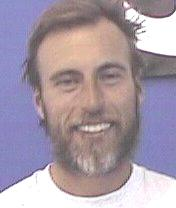
\includegraphics[scale=1.5]{files/matt.jpg}
	\end{minipage}
	\end{exampleblock}
	
	\begin{alertblock}{What is PAQ?}<2->
		\begin{itemize}
			\item A lossless, open-source compression algorithm
			\item Brings high perfomance at the cost of increased memory usage and time consumption
			\item Related to PPM, is envisioned as PPMs improvement
		\end{itemize}
	\end{alertblock}
\end{frame}

\begin{frame}
	\begin{exampleblock}{Principles of PAQ}
	
		\begin{itemize}
			\item Modeling combined with adaptive arithmetic encoding
			\item Open to additions and improvements
			\item Improves perfomance of PPM by including several predictors (i.e. models of data) 
			\item Combines the result of the predictors 
		\end{itemize}
	\end{exampleblock}

\end{frame}

\begin{frame}
	\begin{block}{Exemplary Predictors}
	\visible<1->{The order-$n$ context predictor
		\begin{itemize}
			\item Examines the last $n$ bits and counts the 1's and 0's
			\item Estimates probability whether next bit is 1 or 0 like PPM
		\end{itemize}	
		}		
	\visible<2->{
	The sparse context predictor
		\begin{itemize}
			\item 	Context consists of a specific amount of non-contiguous bytes before the current bit 
		\end{itemize}
		}
	\end{block}
	
	\begin{exampleblock}{PAQ \& Predictors}<3->
		\begin{itemize}
			\item 	Predictors in PAQ are used simultaneously
			\item Result with the most usability is chosen
		\end{itemize}

	\end{exampleblock}
	
\end{frame}

\begin{frame}

\end{frame}


\section{PAQ8}
\subsection{Architecture}
\subsection{Model Mixer}
\subsection{Mixture of Experts}
\subsection{Updating \& Filtering}
\section{Applications for PAQ8}
\section{References}





\end{document}